\chapter{Detailed Design}

% Simply functionality and availability, is selected based on the relative important of these criteria.............. 
Detailed design is the phase where the design is refined and plans, specifications
and estimates are created. Detailed design will include outputs such as 2D and 3D
models, cost build up estimates, procurement plans etc. This phase is where the full
cost of the project is identified.

\section{Data Dictionary}
Data dictionary is only collection of data element definition. Entries in a data dictionary include the name of the data item and attributes. A data dictionary is a file or a set of files that contains a databases metadata. In a relational database, the metadata in the data dictionary includes the following: Names of all tables in the database and their owners. Names of all indexes and the columns to which the tables in those indexes relate. Constraints defined on tables, including primary keys, foreign-key relationships to other tables, and not-null constraints.

% Data dictionary is only collection of data element definition. Entries in a data dictionary include the name of the data item and attributes. ...........

        

% \section{Input and output Design}

% 		Considering all o the interaction of user with the system be in most effective and simplified way.                All the input forms are designed in she user will be able to use them in very eff possibilities needed by the user................
		
		
% 		% This section type your project contents 
\section{Input and Output Design}

\textbf{Input Design}\\
Input design is the process of converting user inputs into a computer-based format. This project requires specific information from users to generate detailed reports. To achieve this, well-organized input data is essential. During the system design phase, the expanded Data Flow Diagram (DFD) identifies logical data flows, data stores, and destinations. Input data is collected and grouped based on similarity, facilitating easier processing.The primary objective of input design is to simplify data entry while minimizing logical errors. In the current system, input is minimal, requiring only a \textbf{username} and \textbf{password} from all types of clients. If these credentials are valid, the client is granted access to the software.\\
\textbf{Output Design}\\
Output design plays a crucial role in enhancing the system’s interaction with users and supporting decision-making processes. Effective output design involves identifying the information needs of users and presenting it in a clear, accessible format.Computer output in this system involves both digital and hard-copy formats. The design considers the selection of output devices based on factors such as response time and printing efficiency.
		
		
\subsection{Admin}
\pagebreak
\textbf{login}
\begin{center}
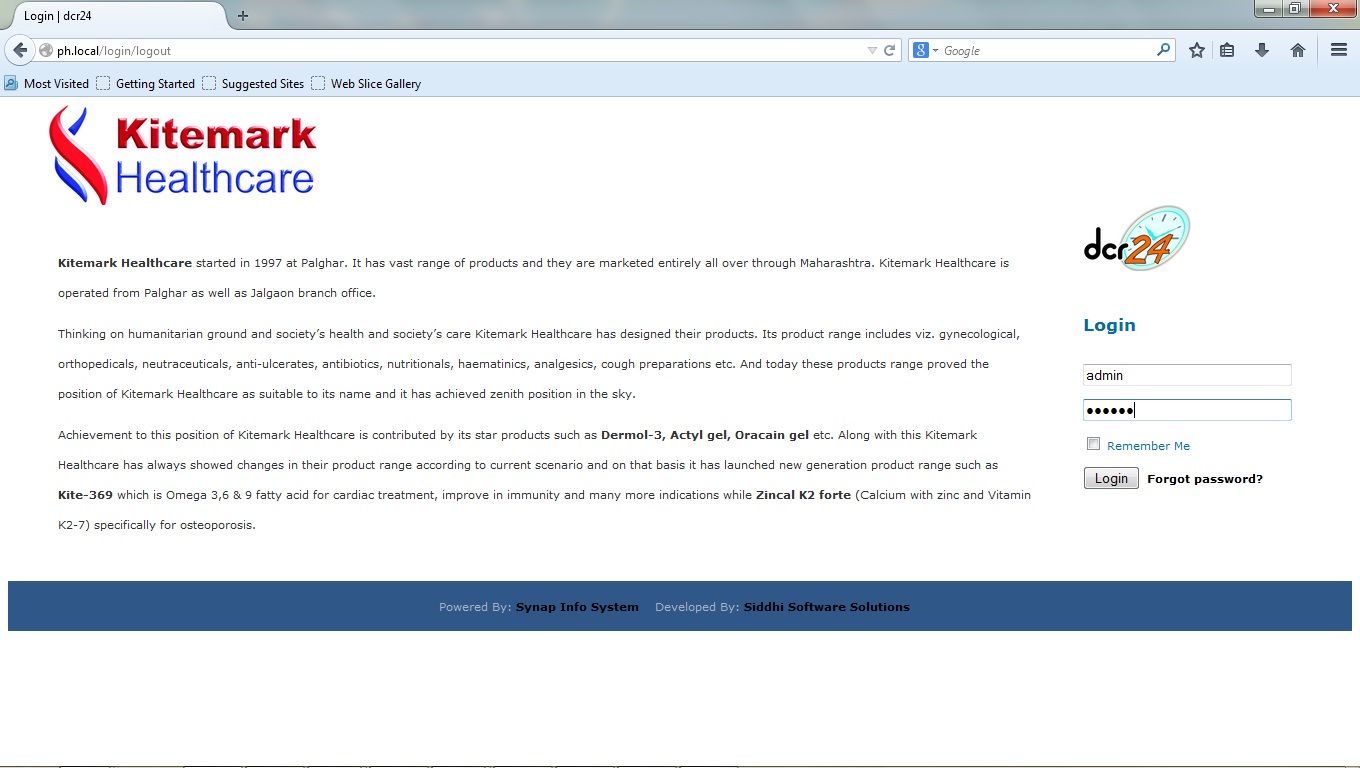
\includegraphics[height=9cm,width=14cm]{Admin/login.jpg}
\end{center}


% This section type your project contents 

\textbf{Admin Dashboard}
\begin{center}
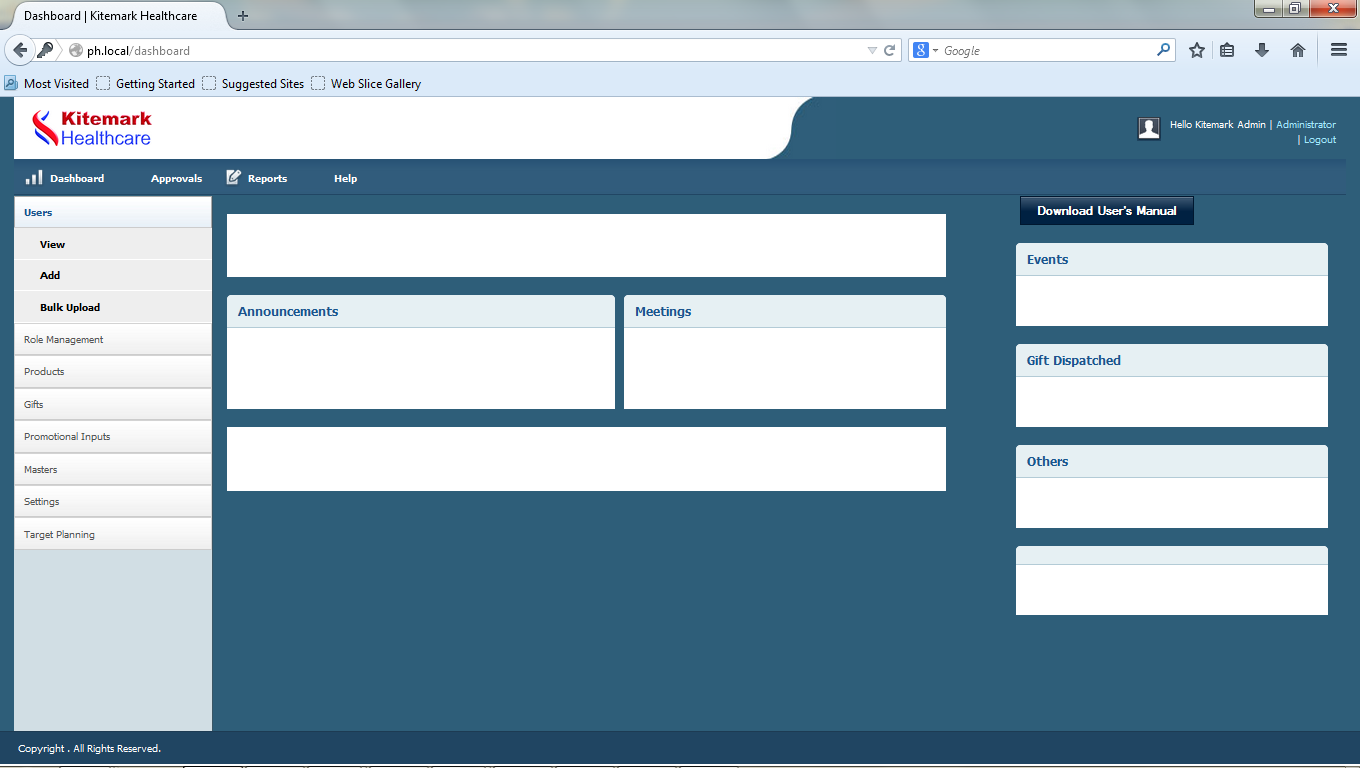
\includegraphics[height=9cm,width=14cm]{Admin/dashboard.png}
\end{center}
\pagebreak

\textbf{View Users}
\begin{center}
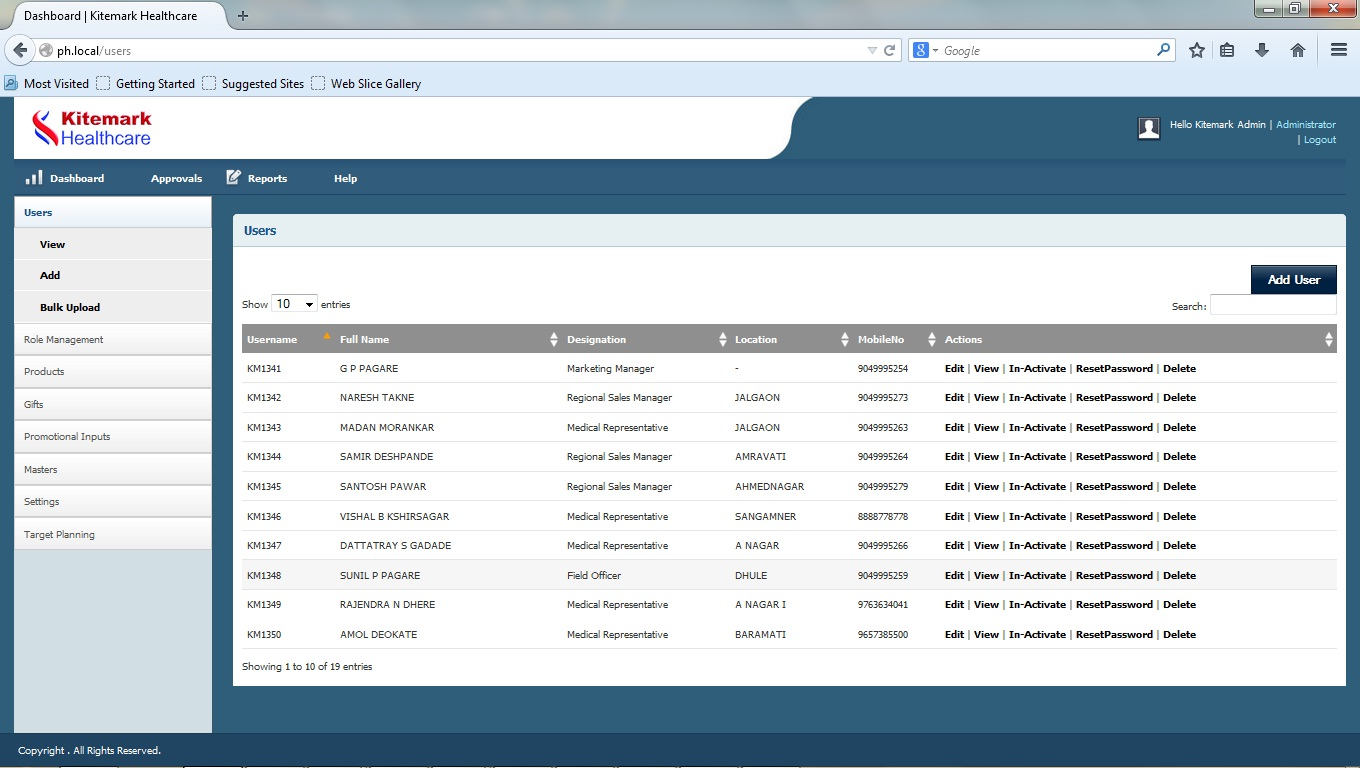
\includegraphics[height=9cm,width=14cm]{Admin/viewusers.jpg}
\end{center}



% This section type your project contents 
\textbf{Add User}
\begin{center}
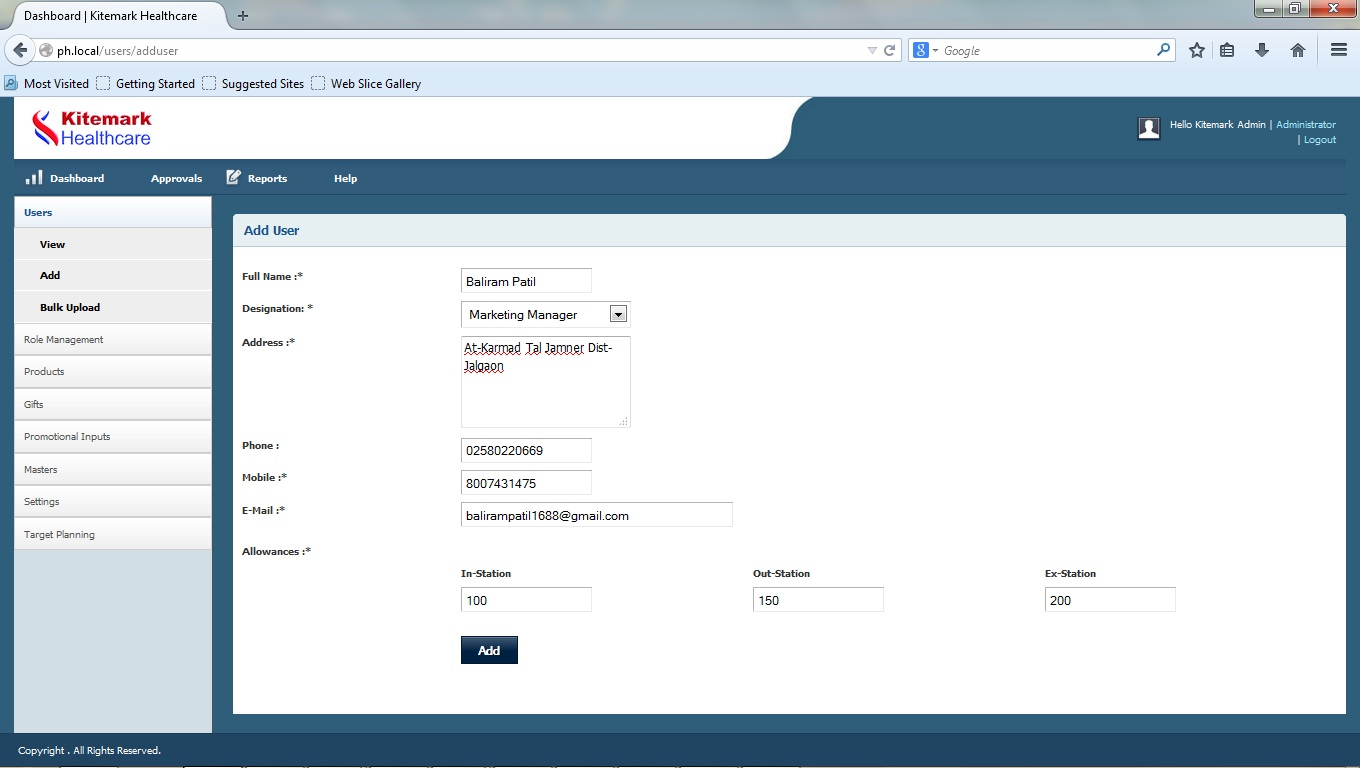
\includegraphics[height=9cm,width=14cm]{Admin/addusers.jpg}
\end{center}
\pagebreak

		
		% This section type your project contents 
		
		
		
		
		
		
		
		
		
		
		
		
		
		
		
		
		
		
		
		
		
		
		
		
		
		
		
 		

\section{Database structure}
\textbf{announcement:}  This table stores announcement added by Admin and useful to display announcement to other users.\nolinebreak
\begin{table}[hp]
\centering

\begin{tabular}{|c|c|c|c|}
\hline
\textbf{Field Name}  & \textbf{Data Type}  & \textbf{size} &\textbf{Constraints}  \\
\hline
announceid & int & 20 & Primary Key,auto\_increment \\
\hline
title &	varchar &	200 & NOT NULL.\\
\hline
description & varchar &	255 & NOT NULL.\\
\hline
addedBy	& int & 11 &	NOT NULL\\
\hline
addedon &	datetime &	- &	NOT NULL.\\
\hline
updatedon &	datetime &	- &	NOT NULL.\\
\hline
expiry\_date & date & 20 & NOT NULL.\\
\hline
status	& varchar &	- & NOT NULL. \\
\hline

\end{tabular}
\caption{ announcement}
\end{table}
\\
\textbf{area:} This table stores area details with region of that area.\nolinebreak
\begin{table}[hp]
\centering
\begin{tabular}{|c|c|c|c|}
\hline
\textbf{Field Name}  & \textbf{Data Type}  & \textbf{size} &\textbf{Constraints}  \\
\hline
area\_id & bigint &	20 & Primary Key,auto\_increment\\
\hline
area &	varchar &	25 & NOT NULL \\
\hline
region\_id &	bigint & 20 & NOT NULL \\
\hline
isActive &	int & 	11  & NOTNULL \\
\hline
addedon & datetime & - & NOT NULL\\
\hline
updatedon &	datetime & - & NOT NULL\\
\hline
\end{tabular}
\caption{area}
\end{table}

\pagebreak
\textbf{chemist:}  This table stores all chemist details added by Medical Representative or Field Officer.\nolinebreak

\begin{table}[hp]
\centering
\begin{tabular}{|c|c|c|c|}
\hline
\textbf{Field Name}  & \textbf{Data Type}  & \textbf{size} &\textbf{Constraints}  \\
\hline
chemist\_id & bigint &	20 & Primary Key,auto\_increment\\
\hline
chemist\_code &	bigint & 20 & NOT NULL\\
\hline
store\_name	& varchar &	100 & NOT NULL\\
\hline
store\_address &	Text &	- & NOT NULL\\
\hline
town\_id & bigint & 	20 & NOT NULL\\
\hline
contact\_person & varchar & 100 & NOT NULL\\
\hline
mobile & varchar & 12 & NOT NULL\\
\hline
email &	varchar & 100 & NOT NULL\\
\hline
dob & date & - & NOT NULL\\
\hline
date\_of\_marrige & date & - & NOT NULL\\
\hline
is\_hospital\_attached & tinyint & 	2 & NOT NULL\\
\hline
hospital\_name &	varchar &	100 & NOT NULL\\
\hline
dr\_of\_hospital &	varchar &	100 & NOT NULL\\
\hline
near\_by\_dr & varchar &	100 & NOT NULL\\
\hline
available\_products &	varchar &	150 & NOT NULL\\
\hline
monthly\_purchase &	bigint & 20 & NOT NULL\\
\hline
status & varchar & 20 & NOT NULL\\
\hline
approved\_by & varchar &	25 & NOT NULL\\
\hline
reject\_reason & varchar & 200 & NOT NULL\\
\hline
added\_by &	bigint & 20 & NOT NULL\\
\hline
added\_on &	datetime &	- & NOT NULL\\
\hline
updated\_by & bigint &	20 & NOT NULL\\
\hline
updated\_on &	datetime &	- & NOT NULL\\
\hline
isActive &	tinyint &	2 & NOT NULL\\
\hline
\end{tabular}
\caption{chemist}
\end{table}


\textbf{target\_product\_sale} This table stores the target of product sales .\nolinebreak
\begin{table}[hp]
\centering
\begin{tabular}{|c|c|c|c|}
\hline
\textbf{Field Name}  & \textbf{Data Type}  & \textbf{size} &\textbf{Constraints}  \\
\hline
id &	bigint &	20 & Primary Key,auto\_increment \\\hline
year &	 int &	11 & NOT NULL \\\hline
hq\_id	 & int &	11 & NOT NULL \\\hline
prod\_id &	bigint &	20 & NOT NULL \\\hline
sale &	double &	- & NOT NULL \\\hline
 added\_by &	bigint &	20 & NOT NULL \\\hline
added\_on &	datetime &	- & NOT NULL \\\hline
updated\_by &	bigint &	20 & NOT NULL \\\hline
updated\_on &	datetime &	- & NOT NULL \\\hline

 
\end{tabular}
\caption{target\_product\_sale}
\end{table}

\textbf{target\_prod\_calculations} This table stores the product wise  target calculation.\nolinebreak
\begin{table}[hp]
\centering
\begin{tabular}{|c|c|c|c|}
\hline
\textbf{Field Name}  & \textbf{Data Type}  & \textbf{size} &\textbf{Constraints}  \\
\hline
id &	bigint &	20 & Primary Key,auto\_increment \\\hline
year &	int &	11 & NOT NULL \\\hline
prod\_id &	bigint &	20 & NOT NULL \\\hline
packing &	varchar &	100 & NOT NULL \\\hline
calc\_value &	double &	- & NOT NULL \\\hline
expected\_growth &	double &	- & NOT NULL \\\hline
min1 &	double &	- & NOT NULL \\\hline
 min2 &	double &	- & NOT NULL \\\hline
  min3 &	double &	- & NOT NULL \\\hline
  added\_by &	bigint &	20 & NOT NULL \\\hline
added\_on &	datetime &	- & NOT NULL \\\hline
updated\_by &	bigint &	20 & NOT NULL \\\hline
updated\_on	 & datetime &	- & NOT NULL \\\hline

 
\end{tabular}
\caption{target\_prod\_calculations}
\end{table}

\textbf{target\_sls} This table stores the  target of sls.\nolinebreak
\begin{table}[hp]
\centering
\begin{tabular}{|c|c|c|c|}
\hline
\textbf{Field Name}  & \textbf{Data Type}  & \textbf{size} &\textbf{Constraints}  \\
\hline
id &	int	 & 11 & Primary Key,auto\_increment \\\hline
month &	text &	 & NOT NULL \\\hline
hq\_id &	int &	11 & NOT NULL \\\hline
product\_id &	int &	11 & NOT NULL \\\hline
sls &	bigint &	20 & NOT NULL \\\hline
closing\_stock &	bigint &	20 & NOT NULL \\\hline
added\_by &	bigint &	20 & NOT NULL \\\hline
added\_on &	datetime &	- & NOT NULL \\\hline
updated\_by &	bigint &	20 & NOT NULL \\\hline
updated\_on &	datetime &	- & NOT NULL \\\hline
monthno &	int &	11 & NOT NULL \\\hline
year &	int &	11 & NOT NULL \\\hline

 
\end{tabular}
\caption{target\_sls}
\end{table}

\pagebreak

\textbf{target\_yearly} This table stores the  yearly target.\nolinebreak
\begin{table}[hp]
\centering
\begin{tabular}{|c|c|c|c|}
\hline
\textbf{Field Name}  & \textbf{Data Type}  & \textbf{size} &\textbf{Constraints}  \\
\hline
id &	int &	11 & Primary Key,auto\_increment \\\hline
year &	  text &	 & NOT NULL \\\hline
hq\_id &	int &	11 & NOT NULL \\\hline
product\_id &	int &	11 & NOT NULL \\\hline
annual\_target &	bigint &	20 & NOT NULL \\\hline
target\_value	& bigint &	20 & NOT NULL \\\hline
intro\_month &	text &	- & NOT NULL \\\hline
added\_by &	bigint &	20 & NOT NULL \\\hline
added\_on &	datetime &	- & NOT NULL \\\hline
updated\_by &	bigint &	20 & NOT NULL \\\hline
updated\_on &	datetime &	- & NOT NULL \\\hline
 
\end{tabular}
\caption{target\_yearly}
\end{table}

\textbf{town} This table stores the  town details.\nolinebreak
\begin{table}[hp]
\centering
\begin{tabular}{|c|c|c|c|}
\hline
\textbf{Field Name}  & \textbf{Data Type}  & \textbf{size} &\textbf{Constraints}  \\
\hline
 town\_id	& bigint &	20 & Primary Key,auto\_increment \\\hline
 town\_code &	bigint	 & 20 & NOT NULL \\\hline
town &	 varchar &	25 & NOT NULL \\\hline
hq\_id &	bigint &	20 & NOT NULL \\\hline
isActive &	tinyint &	11 & NOT NULL \\\hline
status &	varchar &	20 & NOT NULL \\\hline
approved\_by &	varchar &	25 & NOT NULL \\\hline
reject\_reason &	varchar &	200 & NOT NULL \\\hline
added\_by &	bigint &	20 & NOT NULL \\\hline
added\_on &	datetime &	- & NOT NULL \\\hline
updated\_by &	bigint &	20 & NOT NULL \\\hline
updated\_on &	datetime &	- & NOT NULL \\\hline
 
\end{tabular}
\caption{town}
\end{table}

\textbf{users} This table stores the users details.\nolinebreak
\begin{table}[hp]
\centering
\begin{tabular}{|c|c|c|c|}
\hline
\textbf{Field Name}  & \textbf{Data Type}  & \textbf{size} &\textbf{Constraints}  \\
\hline
 id &	int &	11 & Primary Key,auto\_increment \\\hline
company\_code &	varchar &	3 & NOT NULL \\\hline
username &	varchar &	25 & NOT NULL \\\hline
password &	varchar &	25 & NOT NULL \\\hline
fullname &	varchar &	50 & NOT NULL \\\hline
role\_id &	int &	11 & NOT NULL \\\hline
reports\_to &	int &	11 & NOT NULL \\\hline
address &	varchar &	50 & NOT NULL \\\hline
phone &	varchar	 & 25 & NOT NULL \\\hline
mobile &	varchar &	10 & NOT NULL \\\hline
email &	varchar &	50 & NOT NULL \\\hline
nation\_id &	int &	20 & NOT NULL \\\hline
zone\_id &	bigint &	20 & NOT NULL \\\hline
state\_id &	bigint &	20 & NOT NULL \\\hline
division\_id &	bigint &	20 & NOT NULL \\\hline
region\_id &	bigint &	20 & NOT NULL \\\hline
area\_id &	bigint &	20 & NOT NULL \\\hline
headQuarter\_id &	bigint &	20 & NOT NULL \\\hline
based\_on &	varchar &	50 & NOT NULL \\\hline
addedBy &	bigint &	20 & NOT NULL \\\hline
addedOn &	datetime &	- & NOT NULL \\\hline
updatedOn &	datetime &	- & NOT NULL \\\hline
 isActive &	tinyint &	1 & NOT NULL \\\hline
instation &	int &	11 & NOT NULL \\\hline
outstation &	int &	11 & NOT NULL \\\hline
exstation &	int &	11 & NOT NULL \\\hline

\end{tabular}
\caption{users}
\end{table}

\textbf{users\_leave} This table stores the userwise leave details.\nolinebreak
\begin{table}[hp]
\centering
\begin{tabular}{|c|c|c|c|}
\hline
\textbf{Field Name}  & \textbf{Data Type}  & \textbf{size} &\textbf{Constraints}  \\
\hline
user\_id &	int &	11 &  Primary Key,auto\_increment \\\hline
holiday\_id &	int &	11 & NOT NULL \\\hline
date & date &	- & NOT NULL \\\hline

\end{tabular}
\caption{users\_leaves}
\end{table}

\textbf{users\_profile} This table stores the user profiles details.\nolinebreak
\begin{table}[hp]
\centering
\begin{tabular}{|c|c|c|c|}
\hline
\textbf{Field Name}  & \textbf{Data Type}  & \textbf{size} &\textbf{Constraints}  \\
\hline
profile\_id &	int &	11 &  Primary Key,auto\_increment \\\hline
profile\_name &	varchar &	50 & NOT NULL \\\hline
discription  & varchar &	200 & NOT NULL \\\hline

\end{tabular}
\caption{users\_profile}
\end{table}

\pagebreak

\textbf{user\_roles} This table stores the user roles details.\nolinebreak
\begin{table}[hp]
\centering
\begin{tabular}{|c|c|c|c|}
\hline
\textbf{Field Name}  & \textbf{Data Type}  & \textbf{size} &\textbf{Constraints}  \\
\hline
role\_id &	int &	11 & Primary Key,auto\_increment \\\hline
profile\_id &	varchar &	3 & NOT NULL \\\hline
 parent\_id &	varchar &	25 & NOT NULL \\\hline
designation &	varchar &	25 & NOT NULL \\\hline
permission &	varchar &	50 & NOT NULL \\\hline
isActive &	int &	11 & NOT NULL \\\hline
added\_by	 & bigint	& 20 & NOT NULL \\\hline
added\_on	 & datetime &	- & NOT NULL \\\hline
updated\_by &	bigint &	20 & NOT NULL \\\hline
updated\_on &	datetime &	- & NOT NULL \\\hline
  

\end{tabular}
\caption{users\_roles}
\end{table}

\textbf{zones} This table stores the zones details.\nolinebreak
\begin{table}[hp]
\centering
\begin{tabular}{|c|c|c|c|}
\hline
\textbf{Field Name}  & \textbf{Data Type}  & \textbf{size} &\textbf{Constraints}  \\
\hline
zone\_id &	bigint &	20 & Primary Key,auto\_increment \\\hline
title &	varchar &	25 & NOT NULL \\\hline
 nation\_id &	int &	11 & NOT NULL \\\hline
isActive &	 int &	11 & NOT NULL \\\hline
addedOn &	datetime &	- & NOT NULL \\\hline

\end{tabular}
\caption{zones}
\end{table}

